\documentclass[12pt,a4paper]{book}
% \documentclass[a4paper,french]{book}
% \usepackage[17pt]{extsizes}


\usepackage[table,dvipsnames,svgnames]{xcolor}
\usepackage{listingsutf8}
%\usepackage[utf8]{inputenc}% gestion des accents (source)
\usepackage[T1]{fontenc}% gestion des accents (PDF)
\usepackage{fontspec}
\usepackage[french]{babel}% gestion du français
\usepackage{textcomp}% caractères additionnels
\usepackage{mathtools,amssymb,amsthm}% packages de l'AMS + mathtools
\usepackage{amsmath}
\usepackage{yhmath}
\usepackage{mathpazo}
\usepackage[scaled=0.95]{helvet}
\usepackage{courier}
%\usepackage{fourier}
%\usepackage[scaled=0.95]{helvet}
%\usepackage{courier}
\usepackage{bm}
\usepackage{gensymb}
\usepackage{graphicx}

\usepackage{enumitem}
\usepackage{pifont}

\usepackage{pstricks}
\usepackage{pstricks-add}
\usepackage{pst-eucl}
\usepackage{pgfplots}
\let\clipbox\relax
%\usepackage{pst-plot,pst-text,pst-tree,pstricks-add}
%\usepackage{pst-node} % required package
\usepackage{pst-all}
\usepackage[most,skins,breakable]{tcolorbox}

\usepackage{euscript}





% ############### Nouvelles commandes ###############
% Coloration des labels des points dans pst-eucl
\makeatletter
\define@key[psset]{pst-eucl}{LabelColor}{\def\psk@LabelColor{#1}}
\psset{LabelColor=black}
\def\Pst@WhichLabel#1{{\color{\psk@LabelColor}%
		\ifx\psk@PointName\@default#1\else\psk@PointName\fi}}
\makeatother

% renomme le symbole #2 en #1#2 et invalide le symbole initial #2:
\def\renamesymbol#1#2{
	\expandafter\let\expandafter\newsym\expandafter=\csname#2\endcsname
	\expandafter\global\expandafter\let\csname#1#2\endcsname=\newsym
	\expandafter\global\expandafter\let\csname#2\endcsname=\origsym
}



\usepackage{ProfCollege}
\renamesymbol{Casio}{Calculatrice}
\usepackage[nonshellescape]{ProfLycee}



%\usepackage[left=1.5cm,right=1.5cm,top=2.5cm,bottom=2.5cm]{geometry}
\usepackage[left=13mm,right=13mm,top=18mm,bottom=18mm,footskip=30pt]{geometry}
\setlength{\headheight}{15pt}

\usepackage{titlesec}
\usepackage{pas-math}
\usepackage{longtable}
\usepackage{tikz,tkz-tab}
\usepackage{amsmath}
\usepackage[right]{eurosym}
\usepackage{sectsty}
\usepackage{tipfr}
\usepackage{setspace}

%pour faire les touches de la calculatrices
\usepackage{menukeys}
\renewmenumacro{\menu}{roundedmenus} % default: menus
\renewmenumacro{\directory}{pathswithfolder} % default: paths
\renewmenumacro{\keys}{shadowedroundedkeys} % default: roundedkeys


\usepackage{multicol}
\usepackage{multirow}
\usepackage{systeme}

%% Format des titres de chapitres, paragraphes, ...
\titleformat{\chapter}[frame]
{\color{red!85!white}\normalsize}%
{\filright\sffamily\Large%
	\enspace Chapitre \thechapter\enspace}%
{8pt}
{\color{red!85!white}\rule{0pt}{30pt}\sffamily\Huge\bfseries\filcenter}
%%%%%%%%%%%%%%%%%%%%
\titlespacing{\chapter}{0pc}{0pc}{2pc}
\titlespacing{\subsection}{2pc}{}{}

\titleformat{\subsection}[block]{\hspace{1em}}{\thesubsection}{1em .}{}
\titleformat{\subsubsection}[block]{\hspace{2em}}{\thesubsection}{1em )}{}

\chapterfont{\color{red}{}}
\sectionfont{\color{green!55!black}{}}
\subsectionfont{\color{cyan!65!black}{}}
\subsubsectionfont{\color{violet}{}}
\renewcommand{\thesection}{\color{green!55!black}\Roman{section}.}
\renewcommand{\thesubsection}{\color{cyan!65!black}\arabic{subsection})}
\renewcommand{\thesubsubsection}{\color{violet}\alph{subsubsection})}
\setcounter{secnumdepth}{3}

\titleformat{\subsection}[block]{\hspace{1em}}{\thesubsection}{1em .}{}
\titleformat{\subsubsection}[block]{\hspace{2em}}{\thesubsection}{1em )}{}

\usepackage[column=A]{cellspace}
\setlength{\cellspacebottomlimit}{4pt}
\setlength{\cellspacetoplimit}{4pt}
\setlength{\parindent}{2pt}
\setlength{\tabcolsep}{0.5cm}


%entête et pieds de pages
\usepackage{fancyhdr}
\pagestyle{fancy}
\fancyhf{}
\usepackage{lastpage}
\renewcommand{\chaptermark}[1]{\markboth {Chap. \thechapter~ - ~#1}{}}
\renewcommand\headrulewidth{1pt}
\fancyhead[LO,RE]{1ère G - spécialité maths}
\fancyhead[RO,LE]{\leftmark}
\renewcommand\footrulewidth{1pt}
\fancyfoot[LO,RE]{Année 2025-2026}
\fancyfoot[RO,LE]{\textbf{Page \thepage/\pageref{LastPage}}}

%Mes boites pour les définitions, propriétés, remarques, ...

%Mes boites pour les définitions, propriétés, remarques, ...

\newcommand\titrebox[1]{\textbf{#1}}
\newtcolorbox{definition}{breakable,colback=red!10!white,
	colframe=red!85!white, fonttitle=\bfseries,enhanced,
	attach boxed title to top left={xshift=5mm, yshift=-2mm},boxed title style={size=small,colback=red!10!white,colframe=red!85!white, arc=0.5mm},
	title=\textcolor{red!85!white}{Définition} , arc=3mm}

\newtcolorbox{definitionTitre}[1]{breakable,colback=red!10!white,
	colframe=red!85!white, fonttitle=\bfseries,enhanced,
	attach boxed title to top left={xshift=5mm, yshift=-2mm},boxed title style={size=small,colback=red!10!white,colframe=red!85!white, arc=0.5mm},
	title=\textcolor{red!85!white}{Définition - #1} , arc=3mm}

\newtcolorbox{definitionPerso}[1]{breakable,colback=red!10!white,
	colframe=red!85!white, fonttitle=\bfseries,enhanced,
	attach boxed title to top left={xshift=5mm, yshift=-2mm},boxed title style={size=small,colback=red!10!white,colframe=red!85!white, arc=0.5mm},
	title=\textcolor{red!85!white}{#1} , arc=3mm}

\newtcolorbox{regle}{breakable,colback=red!10!white,
	colframe=red!85!white, fonttitle=\bfseries,enhanced,
	attach boxed title to top left={xshift=5mm, yshift=-2mm},boxed title style={size=small,colback=red!10!white,colframe=red!85!white, arc=0.5mm},
	title=\textcolor{red!85!white}{Règle} , arc=3mm}

\newtcolorbox{regles}{breakable,colback=red!10!white,
	colframe=red!85!white, fonttitle=\bfseries,enhanced,
	attach boxed title to top left={xshift=5mm, yshift=-2mm},boxed title style={size=small,colback=red!10!white,colframe=red!85!white, arc=0.5mm},
	title=\textcolor{red!85!white}{Règles} , arc=3mm}

\newtcolorbox{definitions}{breakable,colback=red!10!white,
	colframe=red!85!white, fonttitle=\bfseries,enhanced,
	attach boxed title to top left={xshift=5mm, yshift=-2mm},boxed title style={size=small,colback=red!10!white,colframe=red!85!white, arc=0.5mm},
	title=\textcolor{red!85!white}{Définitions} , arc=3mm}

\newtcolorbox{propriete}{breakable,colback=red!10!white,
	colframe=red!85!white, fonttitle=\bfseries,enhanced,
	attach boxed title to top left={xshift=5mm, yshift=-2mm},boxed title style={size=small,colback=red!10!white,colframe=red!85!white, arc=0.5mm},
	title=\textcolor{red!85!white}{Propriété} , arc=3mm}

\newtcolorbox{proprieteTitre}[1]{breakable,colback=red!10!white,
	colframe=red!85!white, fonttitle=\bfseries,enhanced,
	attach boxed title to top left={xshift=5mm, yshift=-2mm},boxed title style={size=small,colback=red!10!white,colframe=red!85!white, arc=0.5mm},
	title=\textcolor{red!85!white}{Propriété - #1} , arc=3mm}

\newtcolorbox{proprietes}{breakable,colback=red!10!white,
	colframe=red!85!white, fonttitle=\bfseries,enhanced,
	attach boxed title to top left={xshift=5mm, yshift=-2mm},boxed title style={size=small,colback=red!10!white,colframe=red!85!white, arc=0.5mm},
	title=\textcolor{red!85!white}{Propriétés} , arc=3mm}

\newtcolorbox{theoreme}{breakable,colback=red!10!white,
	colframe=red!85!white, fonttitle=\bfseries,enhanced,
	attach boxed title to top left={xshift=5mm, yshift=-2mm},boxed title style={size=small,colback=red!10!white,colframe=red!85!white, arc=0.5mm},
	title=\textcolor{red!85!white}{Théorème} , arc=3mm}

\newtcolorbox{theoremeTitre}[1]{breakable,colback=red!10!white,
	colframe=red!85!white, fonttitle=\bfseries,enhanced,
	attach boxed title to top left={xshift=5mm, yshift=-2mm},boxed title style={size=small,colback=red!10!white,colframe=red!85!white, arc=0.5mm},
	title=\textcolor{red!85!white}{Théorème - #1} , arc=3mm}

\newtcolorbox{theoremes}{breakable,colback=red!10!white,
	colframe=red!85!white, fonttitle=\bfseries,enhanced,
	attach boxed title to top left={xshift=5mm, yshift=-2mm},boxed title style={size=small,colback=red!10!white,colframe=red!85!white, arc=0.5mm},
	title=\textcolor{red!85!white}{Théorèmes} , arc=3mm}

\newtcolorbox{bexemple}{
	enhanced,
	breakable,
	fonttitle=\bfseries,
	frame empty,
	nobeforeafter,
	borderline west={0.5mm}{0mm}{cyan!75!black},
	title=\textcolor{cyan!75!black}{\faHubspot\:\:Exemple},
	%title after break=Exemple (suite),
	colback=white,
	extras={enhanced, frame empty},
	detach title,before upper={\tcbtitle\ :\quad },
}

\newtcolorbox{bexemples}{
	enhanced,
	breakable,
	fonttitle=\bfseries,
	frame empty,
	nobeforeafter,
	borderline west={0.5mm}{0mm}{cyan!75!black},
	title=\textcolor{cyan!75!black}{\faHubspot\:\:Exemples},
	%title after break=Exemples (suite),
	colback=white,
	extras={enhanced, frame empty},
	detach title,before upper={\tcbtitle\ :\quad },
}

\newtcolorbox{bexemplet}[1]{
	enhanced,
	breakable,
	fonttitle=\bfseries,
	frame empty,
	borderline west={0.5mm}{0mm}{cyan!75!black},
	title=\textcolor{cyan!75!black}{\faHubspot\:\:Exemple - #1},
	colback=white,
	extras={enhanced, frame empty},
	detach title,before upper={\tcbtitle\ :\quad },
}

\newtcolorbox{brmq}{
	enhanced,
	breakable,
	fonttitle=\bfseries,
	frame empty,
	nobeforeafter,
	borderline west={0.5mm}{0mm}{orange!95!white},
	title=\textcolor{orange!85!white}{\faHandPointRight[regular]\:\:Remarque} ,
	colback=white,
	extras={enhanced, frame empty},
	detach title,before upper={\tcbtitle\ \quad },
}

\newtcolorbox{brmqs}{
	enhanced,
	breakable,
	fonttitle=\bfseries,
	frame empty,
	nobeforeafter,
	borderline west={0.5mm}{0mm}{orange!85!white},
	title=\textcolor{orange!85!white}{\faHandPointRight[regular]\:\:Remarques},
	colback=white,
	detach title,before upper={\tcbtitle\ \quad },
	extras={enhanced, frame empty},
}

\newtcolorbox{brmqt}[1]{
	enhanced,
	breakable,
	fonttitle=\bfseries,
	frame empty,
	nobeforeafter,
	borderline west={0.5mm}{0mm}{orange!85!white},
	title=\textcolor{orange!85!white}{\faHandPointRight[regular]\:\:Remarque - #1},
	colback=white,
	extras={enhanced, frame empty},
	detach title,before upper={\tcbtitle\ \quad },
}

\newtcolorbox{consequences}[1]{
	enhanced,
	breakable,
	fonttitle=\bfseries,
	frame empty,
	nobeforeafter,
	borderline west={0.5mm}{0mm}{ProcessBlue},
	title=\textcolor{ProcessBlue}{#1},
	colback=white,
	extras={enhanced, frame empty},
	detach title,before upper={\tcbtitle\ :\quad },
}

\newtcolorbox{bmethode}{
	enhanced,
	breakable,
	fonttitle=\bfseries,
	frame empty,
	nobeforeafter,
	borderline west={0.5mm}{0mm}{blue!75!black},
	title=\textcolor{blue!75!black}{Méthode} ,
	colback=white,
	extras={enhanced, frame empty},
	attach boxed title to top left = {xshift = -3mm},
	boxed title style={size=small,colback=white,colframe=blue!75!black, arc=3mm,
	}
}

\newtcolorbox{bmethodes}{
	enhanced,
	breakable,
	fonttitle=\bfseries,
	frame empty,
	nobeforeafter,
	borderline west={0.5mm}{0mm}{blue!75!black},
	title=\textcolor{blue!75!black}{Méthodes} ,
	colback=white,
	extras={enhanced, frame empty},
	attach boxed title to top left = {xshift = -3mm},
	boxed title style={size=small,colback=blue!75!black,colframe=blue!75!black, arc=3mm,
	}
	boxed title after break style={size=small,colback=white,colframe=blue!75!black, arc=3mm,
	}
}

\newtcolorbox{bmethodet}[1]{
	enhanced,
	breakable,
	fonttitle=\bfseries,
	frame empty,
	nobeforeafter,
	borderline west={0.5mm}{0mm}{blue!75!black},
	title=\textcolor{blue!75!black}{\faTasks\:\:Méthode - #1} ,
	colback=white,
	extras={enhanced, frame empty},
	attach boxed title to top left = {xshift = -3mm},
	boxed title style={size=small,colback=white,colframe=blue!75!black, arc=3mm,
	}
}

\newtcolorbox{bdemo}{
	enhanced,
	breakable,
	fonttitle=\bfseries,
	frame empty,
	nobeforeafter,
	borderline west={0.5mm}{0mm}{violet!65!white},
	title={\faEdit[regular]\:\:Démonstration},
	%title after break=Démonstration (suite),
	colback=white,
	extras={enhanced, frame empty},
	attach boxed title to top left = {xshift = -3mm},
	boxed title style={size=small,colback=violet!65!white,colframe=violet!65!white, arc=3mm,
	}
}

\newtcolorbox{bdemos}{
	enhanced,
	breakable,
	fonttitle=\bfseries,
	frame empty,
	nobeforeafter,
	borderline west={0.5mm}{0mm}{violet!65!white},
	title={\faEdit[regular]\:\:Démonstrations},
	%title after break=Démonstration (suite),
	colback=white,
	extras={enhanced, frame empty},
	attach boxed title to top left = {xshift = -3mm},
	boxed title style={size=small,colback=violet!65!white,colframe=violet!65!white, arc=3mm,
	}
}

\newtcolorbox{bdemot}[1]{
	enhanced,
	breakable,
	fonttitle=\bfseries,
	frame empty,
	nobeforeafter,
	borderline west={0.5mm}{0mm}{violet!65!white},
	title={\faEdit[regular]\:\:Démonstration - #1},
	%title after break=Démonstration (suite),
	colback=white,
	extras={enhanced, frame empty},
	attach boxed title to top left = {xshift = -3mm},
	boxed title style={size=small,colback=violet!65!white,colframe=violet!65!white, arc=3mm,
	}
}

\newtcolorbox{boxPerso}[2]{
	enhanced,
	breakable,
	fonttitle=\bfseries,
	frame empty,
	nobeforeafter,
	borderline west={0.5mm}{0mm}{#2},
	title=#1,
	%title after break=Exemple (suite),
	colback=white,
	extras={enhanced, frame empty},
	detach title,before upper={\tcbtitle\ :\quad },
}


\newcommand*{\Coord}[3]{% 
	\ensuremath{\vv{#1}\, 
		\begin{pmatrix} 
			#2\\ 
			#3 
\end{pmatrix}}}

\newcommand*{\CoordSV}[2]{% 
	\ensuremath{\begin{pmatrix} 
			#1\\ 
			#2 
\end{pmatrix}}}

\newcommand*{\Coordp}[3]{% 
	\ensuremath{\vv{#1}\, 
		\left\lvert 
		\begin{matrix} 
			#2\\ 
			#3 
		\end{matrix}  
		\right.% Ne pas oublier le délimiteur invisible. 
}}


%personnalisation des listes non numérotées pour les différentes boites 
\newlist{itemEx}{itemize}{2}
\setlist[itemEx,1]{label=$\bullet$, font=\color{cyan!75!black}}
\setlist[itemEx,2]{label=$\bullet$, font=\color{cyan!75!black}}

\newlist{enumEx}{enumerate}{2}
\setlist[enumEx,1]{label=\arabic*), font=\bf\color{cyan!75!black}}
\setlist[enumEx,2]{label=\alph*), font=\bf\color{cyan!75!black}}

\newlist{itemMet}{itemize}{2}
\setlist[itemMet,1]{label=$\bullet$, font=\color{blue!75!black}}
\setlist[itemMet,2]{label=$\bullet$, font=\color{blue!75!black}}

\newlist{enumMet}{enumerate}{2}
\setlist[enumMet,1]{label=\arabic*), font=\bf\color{blue!75!black}}
\setlist[enumMet,2]{label=\alph*), font=\bf\color{blue!75!black}}

\newlist{itemDef}{itemize}{2}
\setlist[itemDef,1]{label=$\bullet$, font=\color{ForestGreen}}
\setlist[itemDef,2]{label=$\bullet$, font=\color{ForestGreen}}

\newlist{enumDef}{enumerate}{2}
\setlist[enumDef,1]{label=\arabic*), font=\bf\color{ForestGreen}}
\setlist[enumDef,2]{label=\alph*), font=\bf\color{ForestGreen}}

\newlist{itemProp}{itemize}{2}
\setlist[itemProp,1]{label=$\bullet$, font=\color{red!85!white}}
\setlist[itemProp,2]{label=$\bullet$, font=\color{red!85!white}}

\newlist{enumProp}{enumerate}{2}
\setlist[enumProp,1]{label=\arabic*), font=\bf\color{red!85!white}}
\setlist[enumProp,2]{label=\alph*), font=\bf\color{red!85!white}}

\newlist{itemDem}{itemize}{2}
\setlist[itemDem,1]{label=$\bullet$, font=\color{violet!85!white}}
\setlist[itemDem,2]{label=$\bullet$, font=\color{violet!85!white}}

\newlist{enumDem}{enumerate}{2}
\setlist[enumDem,1]{label=\arabic*), font=\bf\color{violet!85!white}}
\setlist[enumDem,2]{label=\alph*), font=\bf\color{violet!85!white}}

\newlist{itemRem}{itemize}{2}
\setlist[itemRem,1]{label=\ding{43}, font=\color{orange!85!white}}
\setlist[itemRem,2]{label=\ding{43}, font=\color{orange!85!white}}

\newlist{enumRem}{enumerate}{2}
\setlist[enumRem,1]{label=\arabic*), font=\bf\color{orange!85!white}}
\setlist[enumRem,2]{label=\alph*), font=\bf\color{orange!85!white}}

% nouvelle commande pour mettre entre guillemets une expression
\newcommand{\guillemets}[1]{\og \emph{#1} \fg}


\newcommand{\corr}[1]{\fcolorbox{red}{yellow!30}{#1}}

\newtcolorbox{corrBox}{enhanced,breakable,boxrule=1pt,nobeforeafter,boxsep=0pt,left=\fboxsep,right=\fboxsep,colback=yellow!30,colframe=red!75!black}

% commandes pour mettre en couleur (et en gras) dans une expression mathématique.
\newcommand{\mVert}[1]{{\color{green!55!black}\bm{#1}}}
\newcommand{\mVertWB}[1]{{\color{green!55!black}#1}}
\newcommand{\mRouge}[1]{{\color{red!85!white}\bm{#1}}}
\newcommand{\mRougeWB}[1]{{\color{red!85!white}#1}}
\newcommand{\mBleu}[1]{{\color{blue!75!black}\bm{#1}}}
\newcommand{\mBleuWB}[1]{{\color{blue!75!black}#1}}
\newcommand{\mOrange}[1]{{\color{orange!75!white}\bm{#1}}}
\newcommand{\mOrangeWB}[1]{{\color{orange!75!white}#1}}
\newcommand{\mViolet}[1]{{\color{violet!85!white}\bm{#1}}}
\newcommand{\mVioletWB}[1]{{\color{violet!85!white}#1}}

%commandes pour les flèches de distributivité.
\newcommand{\tikzmarkBB}[2][]{ \tikz[remember picture, overlay, baseline=-0.5ex]\node[#1, left](#2){}; }
\newcommand{\flechePropV}[4][]{ \tikz[remember picture, overlay]\draw (#2)edge[bend left=90,min distance=1em, -stealth]node[midway, #1]{#4}(#3); }
\newcommand{\flechePropH}[4][]{ \tikz[remember picture, overlay]\draw (#2)edge[bend left=90, min distance=1em, -stealth]node[midway, #1]{#4}(#3); }
\newcommand{\flechePropHbas}[4][]{ \tikz[remember picture, overlay]\draw (#2)edge[bend left=-90, min distance=1em, -stealth]node[midway, #1]{#4}(#3); }


\lstdefinestyle{algo}{%
	inputencoding=utf8,
	mathescape,
	basicstyle=\footnotesize\ttfamily,
	numberstyle=\scriptsize\ttfamily\color{gray},
	showstringspaces=false,
	tabsize=2,
	numbers=left,
	framexleftmargin=8mm,
	xleftmargin=8mm,
	keepspaces=true,
	frame=lines,
	framerule=1pt,
	rulecolor=\color{green!50!black},
	backgroundcolor=\color{green!5},
	keywords = {Pour, allant, Si, alors, Sinon, Fin},    
	morecomment=[l][commentstyle]{//},
	commentstyle=\color{gray},
	classoffset=0,
	keywordstyle=\color{blue!75},
	classoffset=1,
	morekeywords = {Afficher},
	keywordstyle=\color{green!50!black},
	classoffset=0,
	morestring=[b]",
	stringstyle=\color{red!75},
	literate=
	{é}{{\'e}}{1}%
	{è}{{\`e}}{1}%
	{à}{{\`a}}{1}%
	{â}{{\^a}}{1}%%%
	{ç}{{\c{c}}}{1}%
	{œ}{{\oe}}{1}%
	{ù}{{\`u}}{1}%
	{É}{{\'E}}{1}%
	{È}{{\`E}}{1}%
	{À}{{\`A}}{1}%
	{Ç}{{\c{C}}}{1}%
	{Œ}{{\OE}}{1}%
	{Ê}{{\^E}}{1}%
	{ê}{{\^e}}{1}%
	{î}{{\^i}}{1}%
	{ï}{{\"i}}{1}%%%
	{ô}{{\^o}}{1}%
	{û}{{\^u}}{1}%
	{=}{$\leftarrow$}{1}%
	{==}{$={}$}{1}}


%  --------   Macro pour les exercices et leur numérotation  

\newcounter{exo}

\setcounter{exo}{1}

\newcommand{\exercice}[1]{\vskip 0.2cm\noindent{\bf \ Exercice \theexo {  #1 }}\addtocounter{exo}{1}}

\newcounter{rit}

\setcounter{rit}{1}

\newcommand{\rituel}[1]{\vskip 0.2cm\noindent{ \bf \ \underline{Rit. \therit {  #1 }}}\addtocounter{rit}{1}}

\newcommand{\raisedrule}[2][0em]{\leaders\hbox{\rule[#1]{1pt}{#2}}\hfill}

\newcounter{numexo}

\setcounter{numexo}{1}

\newcommand{\exerciceDS}[1]{\vskip 0.6cm\noindent\rule[+2pt]{1cm}{0.5pt}\ {\large\bf \ Exercice \thenumexo {  #1 }}\raisedrule[+2pt]{0.5pt}\null\addtocounter{numexo}{1}\par\vskip 0,4cm}

\newcommand{\bareme}[1]{\tikz\node[circle,draw,inner sep=1pt,outer sep=1pt, color=red]{\textbf{#1}};}

%  --------   Pour le langage Python

% Default fixed font does not support bold face
\DeclareFixedFont{\ttb}{T1}{txtt}{bx}{n}{12} % for bold
\DeclareFixedFont{\ttm}{T1}{txtt}{m}{n}{12}  % for normal

% Custom colors
\usepackage{color}
\definecolor{deepblue}{rgb}{0,0,0.5}
\definecolor{deepred}{rgb}{0.6,0,0}
\definecolor{deepgreen}{rgb}{0,0.5,0}

\usepackage{listings}

% Python style for highlighting
\newcommand\pythonstyle{\lstset{
		language=Python,
		basicstyle=\ttm,
		otherkeywords={self},             % Add keywords here
		keywordstyle=\ttb\color{deepblue},
		emph={MyClass,__init__},          % Custom highlighting
		emphstyle=\ttb\color{deepred},    % Custom highlighting style
		stringstyle=\color{deepgreen},
		frame=tb,                         % Any extra options here
		showstringspaces=false            % 
}}


% Python environment
\lstnewenvironment{python}[1][]
{
	\pythonstyle
	\lstset{#1}
}
{}

% Python for external files
\newcommand\pythonexternal[2][]{{
		\pythonstyle
		\lstinputlisting[#1]{#2}}}

% Python for inline
\newcommand\pythoninline[1]{{\pythonstyle\lstinline!#1!}}


% \begin{document}
	
	% \section{``In-text'' listing highlighting}
	
	% \begin{python}
		% class MyClass(Yourclass):
		%     def __init__(self, my, yours):
		%         bla = '5 1 2 3 4'
		%         print bla
		% \end{python}
	
	% \section{External listing highlighting}
	
	% \pythonexternal{demo.py}
	
	% \section{Inline highlighting}
	
	% Definition \pythoninline{class MyClass} means \dots
	
	% \end{document}

\definecolor{codegreen}{rgb}{0,0.6,0}
\definecolor{codegray}{rgb}{0.5,0.5,0.5}
\definecolor{codepurple}{rgb}{0.58,0,0.82}
\definecolor{backcolour}{rgb}{0.95,0.95,0.92}

\lstdefinestyle{myStyle}{
	backgroundcolor=\color{backcolour},   
	commentstyle=\color{codegreen},
	keywordstyle=\color{magenta},
	numberstyle=\tiny\color{codegray},
	stringstyle=\color{codepurple},
	basicstyle=\ttfamily\footnotesize,
	breakatwhitespace=false,         
	breaklines=true,                 
	captionpos=b,                    
	keepspaces=true,                 
	numbers=left,                    
	numbersep=5pt,                  
	showspaces=false,                
	showstringspaces=false,
	showtabs=false,                  
	tabsize=2
}

\lstset{style=myStyle}

\newcommand{\normeB}[1]{\left\Vert \vv{#1}\right\Vert}

\newcommand\grasmaths[1]{\symbf{#1}}
\newcommand\sfbmath[1]{\symbf{\symsfup{#1}}}
\definecolor{marron}{rgb}{0.64,0.16,0.16}
\definecolor{titrebleu}{rgb}{0,0,0.6}

\usepackage{tabularx}
\usepackage{wasysym}
% ===========================tableaux de base
\newcolumntype{R}[1]{>{\raggedleft\arraybackslash }b{#1}} 
\newcolumntype{L}[1]{>{\raggedright\arraybackslash }b{#1}}
\newcolumntype{C}[1]{>{\centering\arraybackslash }b{#1}}
\newcolumntype{M}[1]{>{\centering\arraybackslash }m{#1}} %doublecentrée
\renewcommand{\tabularxcolumn}[1]{m{#1}}
\newcolumntype{Y}{>{\centering\arraybackslash }X}

%=============================boîtes de cours
\usepackage{fontawesome5}
\newcommand\fontbox{\sffamily}
%\newcommand\titrebox[1]{\textbf{#1}}
\tcbuselibrary{breakable}
\tcbset{bdefaut/.style={%
		fonttitle=\fontbox,%
		enhanced,breakable,center,boxrule=1.25pt,drop shadow=black!33!white,%
		sharp corners=uphill,arc=12pt,before skip=12pt,after skip=12pt,%
		left=5pt,leftupper=5pt,top=1mm,bottom=1mm,%
		before upper=\leavevmode
	}
}
\NewDocumentCommand\bbnewbox{ m m m m O{#4} !O{} }{%nom + titre + icone + bordure/titre/fondtitre + couleur fond + options
	\DeclareTColorBox{#1}{ O{} }{%
		bdefaut,%
		colframe=#4,coltitle=#4!25!Black,colbacktitle=#4!35,colback=#5!10,%
		title={#3\:\:\titrebox{#2##1}},%
		#6
	}%
}

\bbnewbox{bdefi}{Définition}{\faIcon[regular]{comment-dots}}{ForestGreen}
\bbnewbox{bcor}{Corollaire}{\faIcon[regular]{comment-dots}}{ForestGreen}
\bbnewbox{bdefis}{Définitions}{\faIcon[regular]{comment-dots}}{ForestGreen}
\bbnewbox{bhumour}{Humour}{\faIcon[regular]{laugh-wink}}{Yellow}
%\bbnewbox{bprop}{Propriété}{\faCog}{Salmon}
\bbnewbox{bprop}{Propriété}{\faCog}{red!85!white}
\bbnewbox{bprops}{Propriétés}{\faCog}{Salmon}
\bbnewbox{bcscq}{Conséquence}{\faArrowAltCircleRight[regular]}{Salmon}
\bbnewbox{bthm}{Théorème}{\faBullhorn}{FireBrick}
\bbnewbox{blog}{Logiciel}{\faDev}{CornflowerBlue}[white]
\bbnewbox{bhistoire}{Point histoire}{\faUniversity}{Chocolate}[white]

%\bbnewbox{brmq}{Remarque}{\faHandPointRight[regular]}{MidnightBlue}[white]
\bbnewbox{bexercice}{Exercice}{\faHubspot}{MidnightBlue}
%\bbnewbox{bexemple}{Exemple}{\faHubspot}{MediumTurquoise}
\bbnewbox{bvoc}{Vocabulaire}{\faList*[regular]}{YellowGreen}
\bbnewbox{bnota}{Notation}{\faList*}{YellowGreen}
\bbnewbox{bregle}{Règle}{\faList*}{YellowGreen}
\bbnewbox{bcadre}{Cadre}{\faInfoCircle}{Peru}
\bbnewbox{bidee}{Idée}{\faInfo}{LightBlue}
\bbnewbox{bintro}{Intro}{\faMarker}{LightSalmon}
\bbnewbox{billustr}{Illustration}{\faChartLine}{Crimson}[White]
\bbnewbox{bvideo}{}{\faIcon[regular]{file-video}}{teal}[White]
\bbnewbox{bbilan}{Bilan}{\faForward}{Purple}
%\bbnewbox{bmethode}{Méthode}{\faTasks}{Coral}
%\bbnewbox{bmethode}{Méthode}{\faTasks}{blue!75!black}
\bbnewbox{btuto}{Tuto}{\faTerminal}{Coral}[White]
\bbnewbox{bmanip}{Manipulation}{\faCodeBranch}{DarkCyan}[White]
\bbnewbox{bcalco}{Calculatrice}{\faCalculator}{MediumVioletRed}[White]
\bbnewbox{boutil}{Outil}{\faTools}{DeepSkyBlue}[White]
\bbnewbox{basavoir}{À savoir}{\faHeart}{Red}
\bbnewbox{bbloctd}{TD}{\faHourglassStart}{LightSeaGreen}[White]
\bbnewbox{bblocdm}{À vous de jouer}{\faHourglassStart}{LightSeaGreen}[White]
%\bbnewbox{brappel}{Rappel}{\faHandPointUp[regular]}{LightSalmon}
\bbnewbox{brappel}{Rappel}{\faHandPointUp[regular]}{Peru}
\bbnewbox{bresol}{Résolution}{\faPuzzlePiece}{LightSeaGreen}[White]
\bbnewbox{battention}{Attention}{\faExclamationTriangle}{Red}
\bbnewbox{bcode}{Code}{\faCode}{Crimson}[White]
\bbnewbox{bpython}{Python}{\faPython}{SeaGreen}[White]

\newcommand{\grasInDef}[1]{\textcolor{ForestGreen!55!black}{\textbf{#1}}}
\newcommand{\grasInProp}[1]{\textcolor{red!85!white}{\textbf{#1}}}
\newcommand{\grasInEx}[1]{\textcolor{MediumTurquoise!55!black}{\textbf{#1}}}
\newcommand{\grasInRem}[1]{\textcolor{orange!65!white}{\textbf{#1}}}
\newcommand{\grasInMet}[1]{\textcolor{blue!75!black}{\textbf{#1}}}
\newcommand{\grasInDem}[1]{\textcolor{violet!85!white}{\textbf{#1}}}

%\newtcolorbox{bmethodet}[1][]{%
%	bdefaut,%
%	colframe=blue!75!black,coltitle=white,colbacktitle=blue!65!black,colback=blue!75!black!15!white,
%	title={\faTasks\:\:\titrebox{{Méthode - #1}}}
%}

%outil
\newtcolorbox{boutilcalc}[1][]{%
	bdefaut,%
	colframe=DeepSkyBlue,coltitle=black,colbacktitle=DeepSkyBlue!35,colback=White,
	title=\textcolor{DeepSkyBlue!25!Black}{\faFileVideo[regular]\:\:\titrebox{Tuto#1 Vidéo}}
}

%loglogo
\newtcolorbox{bloglogo}[2][]{%
	bdefaut,%
	colframe=CornflowerBlue,coltitle=black,colbacktitle=CornflowerBlue!35,colback=white,
	title=\textcolor{CornflowerBlue!25!Black}{\faDev\:\:\titrebox{Logiciel#1}},
	overlay={\begin{tcbclipinterior}
			\node[opacity=0.33,rotate=-45] at ($(interior.south east)+(-10pt,10pt)$){\includegraphics[height=24pt]{#2}};
	\end{tcbclipinterior}}
}

%demo
%\newtcolorbox{bdemo}[1][]{%
%	bdefaut,%
%	colframe=Violet,coltitle=black,colbacktitle=Violet!35,colback=Violet!15,
%	title=\textcolor{Violet!25!Black}{\faEdit[regular]\:\:\titrebox{Démonstration#1}},
%	overlay={\begin{tcbclipinterior}%
%			\node[] at ($(interior.south east)+(-10pt,10pt)$){\large\textcolor{Violet}{\textbf{\CheckedBox}}};%
%	\end{tcbclipinterior}}
%}


%\newtcolorbox{bdemo}[1][]{%
%	bdefaut,%
%	colframe=violet!85!white,coltitle=black,colbacktitle=Violet!35,colback=Violet!15,
%	title=\textcolor{Violet!25!Black}{\faEdit[regular]\:\:\titrebox{Démonstration#1}},
%	overlay={\begin{tcbclipinterior}%
%			\node[] at ($(interior.south east)+(-10pt,10pt)$){\large\textcolor{Violet}{\textbf{\CheckedBox}}};%
%	\end{tcbclipinterior}}
%}

%demoblanc
\newtcolorbox{bdemoblanc}[1][]{%
	bdefaut,%
	colframe=Violet,coltitle=black,colbacktitle=Violet!35,colback=White,
	title=\textcolor{Violet!25!Black}{\faEdit[regular]\:\:\titrebox{Démonstration#1}},
	overlay={\begin{tcbclipinterior}%
			\node[] at ($(interior.south east)+(-10pt,10pt)$){\large\textcolor{Violet}{\textbf{\CheckedBox}}};%
	\end{tcbclipinterior}}
}

%algo
\newtcolorbox{balgo}[1][]{%
	bdefaut,%
	colframe=OrangeRed,coltitle=black,colbacktitle=OrangeRed!35,colback=White,
	title=\textcolor{OrangeRed!25!Black}{\faFileCode\:\:\titrebox{Algorithme#1}},
	overlay={\begin{tcbclipinterior}%
			\node[opacity=0.15,rotate=-15] at ($(interior.south east)+(-8pt,12pt)$){\includegraphics[height=24pt]{algorithmvec}};%
	\end{tcbclipinterior}}
}


%aide
\newtcolorbox{baide}{%
	bdefaut,%
	colframe=titrebleu!35,coltitle=titrebleu!50!Black,colbacktitle=titrebleu!15,colback=White,
	title=\textcolor{titrebleu!25!Black}{\faBacon\:\:\titrebox{Niveaux de difficulté}},
	overlay={\begin{tcbclipinterior}%
			\node[opacity=0.33,rotate=45,scale=0.33] at ($(interior.south east)+(-6pt,6pt)$){\textcolor{titrebleu!50!Black}{\footnotesize \bfseries \sffamily \textcopyright{} Dairon11}};%
	\end{tcbclipinterior}}
}

\newtcolorbox{bcalcologo}[2][]{%
	bdefaut,%
	colframe=MediumVioletRed,coltitle=black,colbacktitle=MediumVioletRed!35,colback=White,
	title=\textcolor{MediumVioletRed!25!Black}{\faCalculator\:\:\titrebox{Calculatrice#1}},
	overlay={\begin{tcbclipinterior}%
			\node[opacity=0.33,rotate=-45] at ($(interior.south east)+(-10pt,10pt)$){\includegraphics[height=48pt]{#2}};%
	\end{tcbclipinterior}}
}

\definecolor{orangescratch}{HTML}{F8A31F}
\newtcolorbox{bscratch}[1][]{%
	bdefaut,%
	colframe=orangescratch,coltitle=black,colbacktitle=orangescratch!35,colback=White,
	title=\textcolor{orange!25!Black}{\includegraphics[height=1em]{scratch}\:\:\titrebox{Scratch#1}},
	overlay={\begin{tcbclipinterior}%
			\node[opacity=0.33,rotate=45] at ($(interior.south east)+(-12pt,12pt)$){\includegraphics[height=12pt]{scratchban}};%
	\end{tcbclipinterior}}
}

%reponse
\newtcolorbox{breponse}[1][]{%
	bdefaut,%
	colframe=Thistle,coltitle=black,colbacktitle=Thistle!35,colback=White,
	before upper = \vspace{-0.05cm},
	title=\textcolor{Thistle!25!Black}{\faIcon{pen-alt}\:\:\titrebox{Réponse#1}}
}

\usepackage{dashundergaps}
\newcommand\underdash[1][black]{% <- règle la couleur du texte
	\bgroup
	\ifdim\ULdepth=\maxdimen\settodepth\ULdepth{(j}\advance\ULdepth.4pt\fi
	\markoverwith{\kern0.2em% <- règle l'espacement avant un pointillé
		\vtop{\kern0.5ex% <- règle l'altitude des pointillés
			{\color{black}% <- règle la couleur des pointillés
				\hrule width.4em% <- règle la largeur des pointillés
		}}\kern0.2em% <- règle l'espacement après un pointillé
	}\color{#1}\ULon}

\newcommand\pointille[1][1cm]{\makebox[#1]{\dotfill}}



\newcommand{\va}[1]{\lvert \ #1 \ \rvert}
\newcommand{\vaf}[1]{\left\lvert \ #1\  \right\rvert}

\begin{document}
\graphicspath{{images/}}
\setcounter{chapter}{7}
\chapter[Correction des exercices]{Application de la dérivation \\ correction des exercices}
\thispagestyle{fancy}

\subsection*{Ex 17 p 143}
\begin{enumMet}
    \item \ \\
    \begin{tikzpicture}
        \tkzTabInit{$x$ / 1 , $f'(x)$ / 1}{$-2$, $-1$, $2$ ,$4$}
        \tkzTabLine{, -,z , +,z,-,  }
    \end{tikzpicture}
    \item le minimum de $f$ sur $[-2;4]$ est $-2$.\\
    Le maximum de $f$ sur $[-2;4]$ est $3$.\\
\end{enumMet}

\subsection*{Ex 21 p 143}
\begin{tikzpicture}
    \tkzTabInit{$x$ / 1 , $f'(x)$ / 1, $f(x)$ / 2}{$-3$, $-1$, $3$ ,$4$}
    \tkzTabLine{, +,z ,-,z, +,  }
    \tkzTabVar{-/  ,+/$2$,-/$-1$  ,  +/ }
\end{tikzpicture}

\subsection*{Ex 35 p 145}
\begin{enumMet}
    \item $f'(x)=2x+4$\\
    \begin{tikzpicture}
        \tkzTabInit{$x$ / 1 , $f'(x)$ / 1}{$-\infty$, $-2$, $+\infty$}
        \tkzTabLine{, -,z , +,  }
    \end{tikzpicture}
    \item \ \\
    \begin{tikzpicture}
        \tkzTabInit{$x$ / 1 , $f(x)$ / 2}{$-\infty$, $-2$, $+\infty$}
        \tkzTabVar{+/  ,-/$-9$ ,  +/ }
    \end{tikzpicture}
\end{enumMet}





\subsection*{Ex 44 p 147}
\begin{enumMet}
    \item $f$ est une fonction polynôme du troisième degré donc $f$ est définie sur $\mathbb{R}$.
    \item $f$ est une fonction polynôme du troisième degré donc $f$ est dérivable sur $\mathbb{R}$ et
$$
f^{\prime}(x)=-3 x^{2}+3=-3\left(x^{2}-1\right)=-3(x-1)(x+1)
$$
    \item \ \\
    \begin{tikzpicture}
        \tkzTabInit{$x$ / 1 , $f'(x)$ / 1,$f(x)$ / 2}{$-\infty$, $-1$, $1$, $+\infty$}
        \tkzTabLine{, -,z , +,z , -,  }
        \tkzTabVar{+/  ,-/$-2$ ,  +/$2$, -/ }
    \end{tikzpicture}
\end{enumMet}

\subsection*{45 p 147}
\begin{enumMet}
    \item $f$ est une fonction polynôme du troisième degré donc $f$ est définie sur $\mathbb{R}$.
    \item $f$ est une fonction polynôme du troisième degré donc $f$ est dérivable sur $\mathbb{R}$ et $f^{\prime}(x)=3 x^{2}-2 x-1$
    \item $f^{\prime}$ est une fonction trinôme du second degré qui admet deux racines 1 et $-\frac{1}{3}$. De plus le coefficient de $x^{2}$ est positif. La fonction $f$ admet donc le tableau de variations ci-dessous.\\
    \begin{tikzpicture}
        \tkzTabInit{$x$ / 1 , $f'(x)$ / 1,$f(x)$ / 2}{$-\infty$, $-\dfrac{1}{3}$, $1$, $+\infty$}
        \tkzTabLine{, +,z , -,z , +,  }
        \tkzTabVar{-/  ,+/$\dfrac{32}{27}$ ,  -/$0$, +/ }
    \end{tikzpicture}
\end{enumMet}

\subsection*{46 p 147}
\begin{enumMet}
    \item $f$ est une fonction polynôme du quatrième degré donc $f$ est définie sur $\mathbb{R}$.
    \item $f$ est une fonction polynôme du quatrième degré donc $f$ est dérivable sur $\mathbb{R}$ et $f^{\prime}(x)=4 x^{3}-8 \times 2 x=4 x^{3}-16 x=4 x\left(x^{2}-4\right)=4 x(x+2)(x-2)$
    \item On trouve tout d'abord le tableau de signe de $f^{\prime}(x)$ :\\
    \begin{tikzpicture}
        \tkzTabInit{$x$ / 1 , $4x$ / 1,$x+2$ / 1,$x-2$ / 1, $f'(x)$ / 1}{$-\infty$, $-2$, $0$,$2$, $+\infty$}
        \tkzTabLine{, -,t , -,z , +,t,+,  }
        \tkzTabLine{, -,z , +,t , +,t,+,  }
        \tkzTabLine{, -,t , -,t , -,z,+,  }
        \tkzTabLine{, -,z , +,z , -,z,+,  }
    \end{tikzpicture}
    
    Et on peut alors en déduire le tableau de variations de $f$:\\
    \begin{tikzpicture}
        \tkzTabInit{$x$ / 1 , $f'(x)$ / 1,$f(x)$ / 2}{$-\infty$, $-2$, $0$,$2$, $+\infty$}
        \tkzTabLine{, -,z , +,z , -,z,+,  }
        \tkzTabVar{+/  ,-/$-8$ ,  +/$8$,-/$-8$, +/ }
    \end{tikzpicture}
\end{enumMet}


\subsection*{47 p 147}
\begin{enumMet}
    \item $f$ existe pour $x-1 \neq 0$ c'est à dire $x \neq 1 . f$ est donc définie sur $\mathbb{R}-\{1\}$.
    \item $f$ est une fonction rationnelle donc $f$ est dérivable sur $]-\infty ; 1[$ et sur $] 1 ;+\infty[$. On alors $f=\dfrac{u}{v}$ donc $f^{\prime}=\dfrac{u^{\prime} v-v^{\prime} u}{v^{2}}$ ce qui nous donne
$f^{\prime}(x)=\dfrac{x-1-x-2}{(x-1)^{2}}=\dfrac{-3}{(x-1)^{2}} .$
    \item Pour tout $x \neq 1$, $(x-1)^{2}>0$ donc $f^{\prime}(x)<0$. On obtient donc :\\
    \begin{tikzpicture}
        \tkzTabInit{$x$ / 1 , $f'(x)$ / 1,$f(x)$ / 2}{$-\infty$, $1$, $+\infty$}
        \tkzTabLine{, -,d , -,  }
        \tkzTabVar{+/  ,-D+/ ,  -/ }
    \end{tikzpicture}
\end{enumMet}

\subsection*{48 p 147}
\begin{enumMet}
    \item Pour tout $x \in \mathbb{R}, x^{2}+1>0$ donc $f$ est définie sur $\mathbb{R}$. $f=\dfrac{u}{v}$
    \item $f$ est une fonction rationnelle donc $f$ est dérivable sur $\mathbb{R}$ et comme $v$ alors $f^{\prime}=\dfrac{u^{\prime} v-v^{\prime} u}{v^{2}}$ et donc
    $f^{\prime}(x)=\dfrac{-4 x^{2}-4+8 x^{2}}{\left(x^{2}+1\right)^{2}}=\dfrac{4 x^{2}-4}{\left(x^{2}+1\right)^{2}}=\dfrac{4(x+1)(x-1)}{\left(x^{2}+1\right)^{2}}$
    \item $f^{\prime}(x)$ a le même signe que le produit $(x+1)(x-1)$. On obtient donc :
\end{enumMet}

\subsection*{Ex 59 à 63}
\grasInMet{On suppose que $f$ est une fonction définie et dérivable sur un intervalle donné. Déterminer les éventuels extremums locaux de la fonction $f$ sur cet intervalle.}

\subsection*{Ex 59 p 148}
\grasInMet{$f(x)=x^{2}+4 x+3$ sur \R}\\
On a $f'(x)=2 x+4, f'$ est une fonction affine qui s'annule pour $x=-2$. Le tableau de variations de la fonction $f$ est donc:\\
\begin{tikzpicture}
        \tkzTabInit{$x$ / 1 , $f'(x)$ / 1,$f(x)$ / 2}{$-\infty$, $-2$, $+\infty$}
        \tkzTabLine{, -,z , +,  }
        \tkzTabVar{+/  ,-/$-1$, +/ }
    \end{tikzpicture}\\
$f'$ s'annule en changeant de signe pour $x=-2$ donc $f(-2)=-1$ est un minimum local de $f$

\subsection*{60 p 148}
\grasInMet{$f(x)=\frac{1}{4} x\left(x^{2}-12\right)$ sur \R}\\
$$
\text { Comme }f(x)=\frac{1}{4}\left(x^{3}-12 x\right) \text { alors } f^{\prime}(x)=\frac{1}{4}\left(3 x^{2}-12\right)=\frac{3}{4}\left(x^{2}-4\right)=\frac{3}{4}(x+2)(x-2) \text { . }
$$
On obtient alors le tableau de variations ci-dessous.\\
\begin{tikzpicture}
        \tkzTabInit{$x$ / 1 , $f'(x)$ / 1,$f(x)$ / 2}{$-\infty$, $-2$, $2$, $+\infty$}
        \tkzTabLine{, +,z , -,z,+,  }
        \tkzTabVar{-/  ,+/$4$ ,  -/$-4$ , +/ }
    \end{tikzpicture}\\
    $f^{\prime}$ s'annule deux fois en changeant de signe : pour $x=-2$ et pour $x=2 . f(-2)=4$ est un maximum local de $f . f(2)=-4$ est un minimum local de $f$

\subsection*{61 p 148}
\grasInMet{$f(x)=2 x-3+\frac{2}{x-1}$ sur $] 1 ;+\infty[$}\\
On a $f^{\prime}(x)=2-\dfrac{2}{(x-1)^{2}}=\dfrac{2 x^{2}-4 x}{(x-1)^{2}}=\dfrac{2 x(x-2)}{(x-1)^{2}}$
Sur $] 1 ;+\infty\left[(x-1)^{2}>0\right.$. \\
On étudie donc le signe de $2 x(x-2)$ sur $] 1 ;+\infty[$\\
    \begin{tikzpicture}
        \tkzTabInit{$x$ / 1 , $f'(x)$ / 1,$f(x)$ / 2}{$1$, $2$, $+\infty$}
        \tkzTabLine{d, -,z , +,  }
        \tkzTabVar{D+/  ,-/$3$ ,  +/ }
    \end{tikzpicture}\\
    $f^{\prime}$ s'annule en changeant de signe pour $x=2: f(2)=3$ est un minimum local de $f$.


\subsection*{62 p 148}
\grasInMet{$f(x)=-x^{3}+2 x^{2}-2 x+1$ sur \R.}\\
On a $f^{\prime}(x)=-3 x^{2}+4 x-2$ donc $f^{\prime}$ est un trinôme du second degré. De plus son discriminant $\Delta=4^{2}-4 \times 2 \times 3=-8$ et le coefficient devant $x^{2}$ est négatif, donc $f^{\prime}$ est strictement négative sur $\mathbb{R}$. Et donc $f$ est strictement décroissante sur $\mathbb{R}$, donc $f$ n'admet pas d'extremums locaux.

\subsection*{63 p 148}
\grasInMet{$f(x)=\dfrac{3-x}{x-2} \text { sur }]-\infty ; 2[$}\\
$f$ est de la forme $f=\dfrac{u}{v}$ donc $f^{\prime}=\dfrac{u^{\prime} v-v^{\prime} u}{v^{2}}$ d'où $f^{\prime}(x)=\dfrac{-x+2-3+x}{(x-2)^{2}}=\dfrac{-1}{(x-2)^{2}}$.
Pour tout $x \in]-\infty ; 2\left[, f^{\prime}(x)<0\right.$ donc $f$ est strictement décroissante sur $]-\infty ; 2[$ et donc $f$ n'admet pas d'extremum sur $]-\infty ; 2[$.


% \subsection*{50 p 147}
% \begin{enumMet}
%     \item $D_f=\R\backslash\{2\}$
%     \item $f$ est la somme d'une fonction affine et d'une fonction rationnelle donc $f$ est dérivable sur ]$-\infty ; 2[$ et sur $] 2 ;+\infty[$\\ $f$ s'écrit sous la forme $f=u+\dfrac{4}{v}$ donc $f^{\prime}=u^{\prime}+\dfrac{-4 v^{\prime}}{v^{2}}$ et donc\\ $f^{\prime}(x)=1+\dfrac{-4}{(x-2)^{2}}=\dfrac{x^{2}-4 x}{(x-2)^{2}}=\dfrac{x(x-4)}{(x-2)^{2}}$
%     \item Pour tout $x \neq 2, f^{\prime}(x)$ a le même signe que le produit $x(x-4)$. On a donc \\
%     \begin{tikzpicture}
%         \tkzTabInit{$x$ / 1 , $f'(x)$ / 1,$f(x)$ / 2}{$-\infty$, $0$, $2$,$4$, $+\infty$}
%         \tkzTabLine{, +,z , -,d , -,z,+,  }
%         \tkzTabVar{-/  ,+/$-3$ ,  -D+/ ,-/$5$, +/ }
%     \end{tikzpicture}
% \end{enumMet}

% \subsection*{51 p 247}
% \begin{enumMet}
%     \item $D_f=\R\backslash\{-1\}$
%     \item $f'(x)= \dfrac{u'v-v'u}{v^2}=\dfrac{2x(x+1)-1(x^2+3)}{(x+1)^2}=\dfrac{2x^2+2x-x^2-3}{(x+1)^2}=\dfrac{x^2+2x-3}{(x+1)^2}$\\
%     $\dfrac{(x-1)(x+3)}{(x+1)^2}=\dfrac{x^2-1x+3x-3}{(x+1)^2}=\dfrac{x^2+2x-3}{(x+1)^2}=f'(x)$
%     \item \ \\
%     \begin{tikzpicture}
%         \tkzTabInit{$x$ / 1 , $f'(x)$ / 1,$f(x)$ / 2}{$-\infty$, $-3$, $-1$,$1$, $+\infty$}
%         \tkzTabLine{, +,z , -,d , -,z,+,  }
%         \tkzTabVar{-/  ,+/$-6$ ,  -D+/ ,-/$2$, +/ }
%     \end{tikzpicture}
% \end{enumMet}

\subsection*{87 p 151}
\grasInMet{Une entreprise fabrique des rétroviseurs pour voitures. La fonction "coût total" est définie sur $\mathrm{I}=[0 ; 11]$ par $\mathrm{C}(x)=0,3 x^{3}-3 x^{2}+$ $9 x+6$.
$\mathrm{C}(x)$ est exprimée en millier d'euros et $x$ est le nombre de milliers d'articles fabriqués. Le prix de vente de 1000 articles est $8025 $\EUR{}. On suppose que chaque article fabriqué est vendu. La courbe représentative de la fonction $\mathrm{C}$ est représentée ci-dessous dans un repère orthogonal.}
\begin{center}
            \psset{xunit=1.0cm,yunit=0.08cm,algebraic=true,dimen=middle,dotstyle=o,dotsize=5pt 0,linewidth=1.6pt,arrowsize=3pt 2,arrowinset=0.25}
            \begin{pspicture*}(-2.14,-10)(11.7,148)
                \def\C{0.3*x*x*x-3*x*x+9*x+6}
                \def\R{8.025*x}
                \def\B{-0.3*x*x*x+3*x*x-0.975*x-6}
                %\def\B{-0.3*x*x*x*x+3*x*x*x-0.975*x*x-6*x}
                \psgrid[gridcolor=lightgray, subgriddiv=2, gridlabels=0pt,xunit=1,yunit=20](-2.14,-5)(11.7,148)
                \psaxes[labelFontSize=\scriptstyle,xAxis=true,yAxis=true,Dx=1.,Dy=20.,ticksize=-2pt 0,subticks=2]{->}(0,0)(-2.14,-5)(11.7,148)
                \psplot[linecolor=red,linewidth=1.5pt]{0}{11}{\C}
                \psplot[linecolor=blue,linewidth=1.5pt]{0}{11}{\R}
                \psplot[linecolor=violet,linewidth=1.5pt]{0}{11}{\B}
                \begin{scriptsize}
                    \rput[bl](10,140){\large{\red{$C(x)$}}}
                    \rput[bl](10,70){\large{\blue{$R(x)$}}}
                    \rput[bl](9.5,10){\large{\textcolor{violet}{$B(x)$}}}
                \end{scriptsize}
            \end{pspicture*}
            %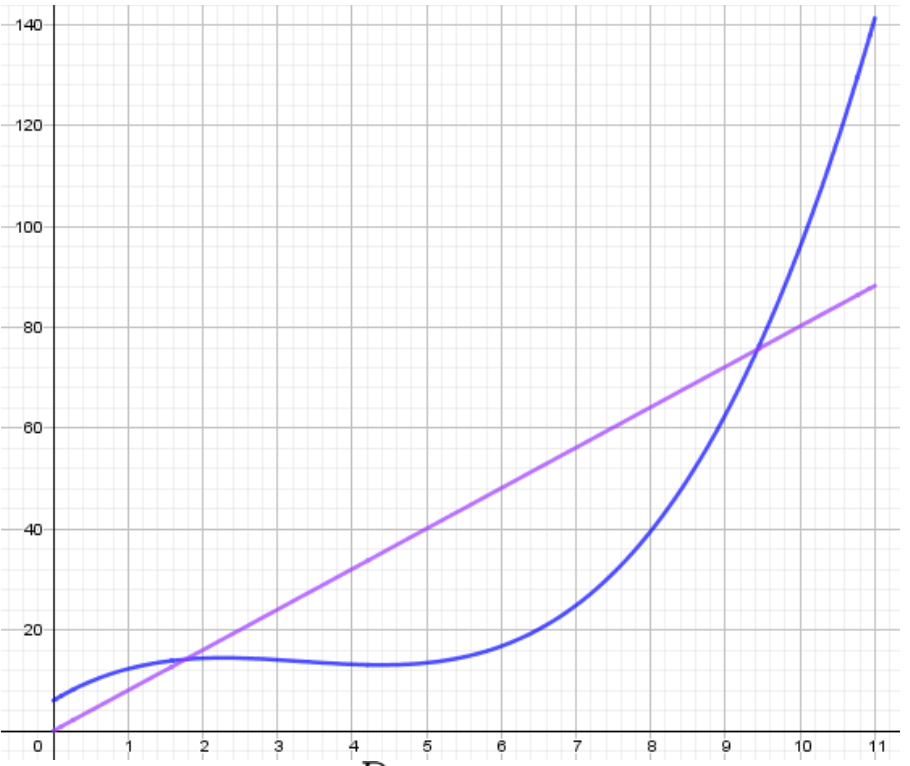
\includegraphics[scale=0.8]{1.08.EXO.Img01}
        \end{center}
\begin{enumMet}
    \item \grasInMet{On note $\mathrm{R}$ la fonction recette, exprimée en millier d'euros, relative à la vente de $x$ milliers d'articles.}
    \begin{enumMet}
        \item \grasInMet{Expliquer pourquoi $\mathrm{R}(x)=8,025 x$.}\\
        Chaque article est vendu 8,025 euro, donc 1000 articles sont vendus 8025 euro soit 8,025 milliers d'euros, d'où $R(x)=8,025 x$.
        \item \grasInMet{Dans le repère ci-dessus, tracer la courbe représentative de $R$.}\\
    On obtient les courbes ci-dessous. La droite bleue est celle de $R$ et la courbe rouge celle de $C$. La courbe violette est celle du bénéfice.
        \item \grasInMet{Déterminer graphiquement l'intervalle de production qui permet de réaliser un bénéfice.}\\
    La courbe représentative de $R$ est au-dessus de la courbe représentative de $C$ pour $x$ compris entre 1,8 et 9,4 (environ) soit une production comprise entre 1800 et 9400 articles.
        \item \grasInMet{Déterminer graphiquement la quantité $x_{0}$ que l'entreprise doit fabriquer pour réaliser un bénéfice maximal.}\\
        L'écart entre les deux courbes entre 1,8 et 9,4 est maximal pour $x \approx 6$, donc le bénéfice est maximal pour une production de 6000 articles environ.
    \end{enumMet}
    \item \grasInMet{Le bénéfice réalisé par cette entreprise est donné, en millier d'euros, par la fonction $\mathrm{B}$ définie et dérivable sur $\mathrm{I}$. On note $\mathrm{B}^{\prime}$ la fonction dérivée de $B$.}
    \begin{enumMet}
        \item \grasInMet{Montrer que, pour tout $x \in \mathrm{I}, \mathrm{B}^{\prime}(x)=-0,075(6 x-1)(2 x-13)$.}\\
    Le bénéfice est donné par $B=R-C$ donc
    $$
    B(x)=8,025 x-0,3 x^{3}+3 x^{2}-9 x-6=-0,3 x^{3}+3 x^{2}-0,975 x-6
    $$
    Et donc $B^{\prime}(x)=-0,3 \times 3 x^{2}+3 \times 2 x-0,975=-0,9 x^{2}+6 x-0,975$.\\
    En développant $-0,075(6 x-1)(2 x-13)$ on obtient $-0,9 x^{2}+6 x-0,975$ donc $B^{\prime}(x)=-0,075(6 x-1)(2 x-13)$
            \item \grasInMet{Étudier le signe de $\mathrm{B}^{\prime}(x)$ puis dresser le tableau de variations de $\mathrm{B}$.}\\
            $B^{\prime}$ est un polynôme du second degré qui a deux racines $x_{1}=\dfrac{1}{6}$ et $x_{2}=6,5$ donc
    $B^{\prime}(x)$ est positif sur $[1 ; 6,5]$ et négatif sur $[6,5 ; 11]$. Et donc $B$ est croissante sur $[1 ; 6,5]$ et décroissante sur $[6,5 ; 11]$\\
    \begin{tikzpicture}
        \tkzTabInit{$x$ / 1 , $f'(x)$ / 1,$f(x)$ / 2}{$1$, $6{,}5$, $11$}
        \tkzTabLine{, +,z , -,  }
        \tkzTabVar{-/  ,+/$32{,}025$, -/ }
    \end{tikzpicture}
    \item \grasInMet{Retrouver, à partir du tableau de variations, la valeur de $x_{0}$.}\\
    La fonction $B$ atteint son maximum pour $x_{0}=6,5$ donc le bénéfice est maximal pour une production de 6500 articles. 
    \item \grasInMet{Quel est le montant, en euro, du bénéfice maximal?}\\
    $B(6,5)=32,025$ donc le bénéfice maximal est de 32025 euros.
    \end{enumMet}
\end{enumMet}

\subsection*{88 p 152}
\grasInMet{D'après Bac technologique - France Métropolitaine - 2009\\
Dans le Périgord, un producteur de truffes noires cultive, ramasse et conditionne de 0 à $45 \mathrm{~kg}$ de ce produit par semaine durant la période de production de la truffe.
On désigne par $x$ le nombre de kilogrammes de truffes traitées chaque semaine et par $f(x)$ le coût unitaire de revient en euro. Chaque kilogramme de truffes conditionné est vendu $450$\EUR{}.
On admet dans la suite du problème que la fonction $f$ est définie sur ] $0 ; 45]$ par $f(x)=x^{2}-60 x+975$}
\begin{enumMet}
    \item \grasInMet{Justifier que le coût de production total $C(x)$ pour $x \mathrm{~kg}$ de truffes est $\mathrm{C}(x)=x^{3}-60 x^{2}+975 x$.}\\
    $f$ correspond au cout de revient unitaire en euro, or le producteur en cultive $x$ kg donc le cout total vaut $C(x)=x f(x)=x^{3}-60 x^{2}+975 x$.
    \item \grasInMet{Exprimer le bénéfice $\mathrm{B}(x)$ réalisé par le producteur pour $x \mathrm{~kg}$ de truffes conditionnés et vendus.}\\
    $B(x)=R(x)-C(x)=450 x-x^{3}+60 x^{2}-975 x$ donc $B(x)=-x^{3}+60 x^{2}-525 x$
    \item \grasInMet{Déterminer la fonction dérivée $\mathrm{B}^{\prime}$ de la fonction $\mathrm{B}$ et montrer que, pour tout $x \in] 0 ; 45], \mathrm{B}^{\prime}(x)=(-3 x+15)(x-35)$.}\\
    On $B^{\prime}(x)=-3 x^{2}+60 \times 2 x-525 x=-3 x^{2}+120 x-525$. En développant $(-3 x+15)(x-35)$ on obtient $-3 x^{2}+120 x-525$ donc $B^{\prime}(x)=(-3 x+15)(x-35)$
    \item \grasInMet{Étudier le signe de $\mathrm{B}^{\prime}(x)$ puis dresser le tableau de variations de $\mathrm{B}$.}\\
    $B^{\prime}$ est un polynôme du second degré admettant deux racines : 5 et 35. Sur $\left.] 0 ; 5\right]$ et sur $[35 ; 45], B^{\prime}(x)$ est négatif et donc $B$ est décroissante. Sur $[5 ; 35], B^{\prime}(x)$ est positif et donc $B$ est croissante. On obtient donc le tableau de variations ci-dessous.\\
    \begin{tikzpicture}
        \tkzTabInit{$x$ / 1 , $B'(x)$ / 1,$B(x)$ / 2}{$0$, $5$,$35$, $45$}
        \tkzTabLine{, -,z , +,z,-,  }
        \tkzTabVar{+/$0$  ,-/$-1250$, +/$12250$, -/$6750$ }
    \end{tikzpicture}
    \item \grasInMet{Compléter le tableau de valeurs suivant:}\\
    Le tableau - une fois complété - est le suivant.\\
    {\setlength{\tabcolsep}{8pt}
    \begin{tabular}{|Xc|Xc|Xc|Xc|Xc|Xc|Xc|Xc|Xc|Xc|Xc|}
    \hline$x$ & 0 & 5 & 10 & 15 & 20 & 25 & 30 & 35 & 40 & 45 \\
    \hline$B(x)$ & 0 & $-1250$ & $-250$ & 2250 & 5500 & 8750 & 11250 & 12250 & 1100 & 6750 \\
    \hline
    \end{tabular}}
    \item On obtient la courbe ci-dessous\\
    \begin{center}
        \psset{xunit=0.27cm,yunit=0.0008cm,algebraic=true,dimen=middle,dotstyle=o,dotsize=5pt 0,linewidth=1.6pt,arrowsize=3pt 2,arrowinset=0.25}
        \begin{pspicture*}(-5.14,-2000)(46,12800)
            \def\B{-x*x*x+60*x*x-525*x}
            \psgrid[gridcolor=lightgray, subgriddiv=2, gridlabels=0pt,xunit=5,yunit=2000](-5.14,-2000)(46,12800)
            \psaxes[labelFontSize=\scriptstyle,xAxis=true,yAxis=true,Dx=5.,Dy=2000.,ticksize=-2pt 0,subticks=2]{->}(0,0)(-5.14,-2000)(46,12800)
            \psplot[linecolor=blue,linewidth=1.5pt]{0}{45}{\B}
            \begin{scriptsize}
                \rput[bl](38,8000){\large{\blue{$B(x)$}}}
            \end{scriptsize}
        \end{pspicture*}
        %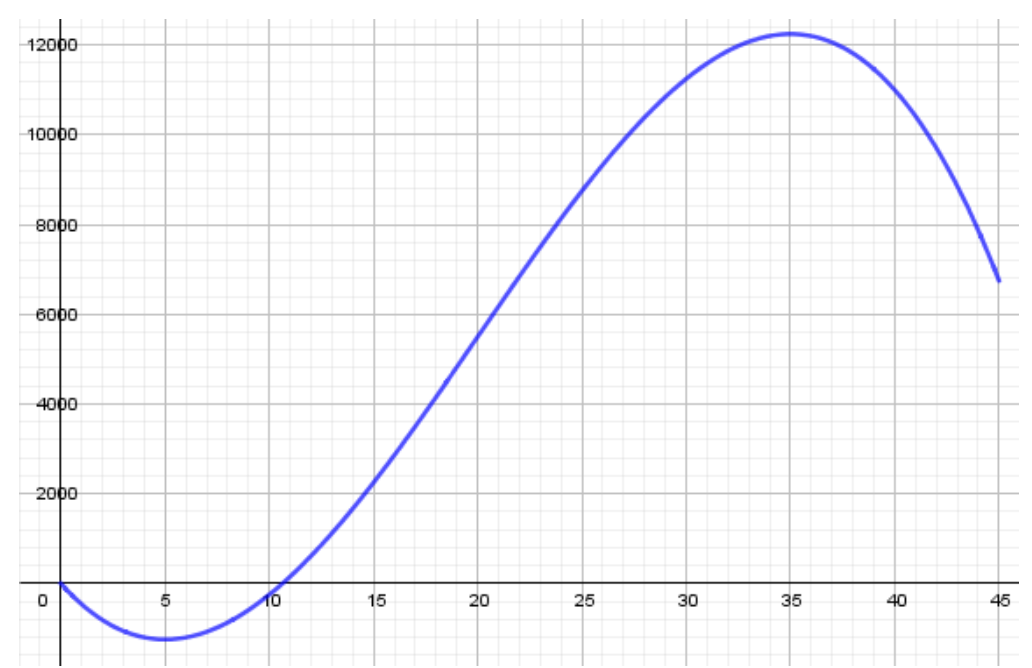
\includegraphics[scale=0.8]{1.08.EXO.Img02}
    \end{center}
\end{enumMet}



% \subsection*{******}
% \begin{enumMet}
%     \item 
% \end{enumMet}

\end{document}

